

%Set default listings style
\lstset{
    basicstyle=\ttfamily\footnotesize,  % Font style and size
    backgroundcolor=\color{codegray},   % Background color
    frame=single,                       % Single-line frame
    framerule=0.4pt,                    % Frame line thickness
    framesep=5pt,                       % Space between frame and code
    captionpos=b,                       % Caption position below the code
    breaklines=true,                    % Enable line breaking if code is too long
    numbers=left,                       % Line numbers on the left side
    numberstyle=\color{gray},      % Style of line numbers
    stepnumber=1,                       % Number lines every 1 line
    numbersep=5pt,                      % Space between line numbers and code
    tabsize=2,                          % Tab size
    showstringspaces=false,            % Do not replace spaces in strings with symbols
}


\section{STORE PROCEDURE/ FUNCTION/ TRIGGER}
\subsection{Store Procedure/ Function}
Trong database bao gồm nhiều procedure, một trong những procedure:\\
GetProductList Proceduce dùng để lấy thông tin của tất cả sản phẩm.

\begin{lstlisting}[language=SQL, caption=GetProductList Procedure] 
CREATE DEFINER=`TranLuongYenNhi`@`%` PROCEDURE `GetProductList`()
BEGIN
    SELECT
        p.ID,
        p.Name,
        p.Description,
        p.Origin,
        p.Tag,
        p.Storage_Condition,
        p.`Country of origin`,
        p.Price,
        p.`Directions for use`,
        p.Certificate,
        p.Warning,
        p.`Intended User`,
        p.`Total amount from batch`,
        c.Ingredient,
        c.Serving_size,
        c.Dosage,
        c.Dosage_form,
        c.Constraindication,
        m.Side_effect,
        m.Indication,
        m.Is_Prescription_Medicine,
        s.Allergen_info,
        me.Usage_Instruction,
        me.Material,
        me.`Size/Dimension`,
        me.Requirement,
        me.Warranty,
        me.Sterility,
        CASE
            WHEN me.ID IS NOT NULL THEN 'medical_equipment'
            WHEN m.ID IS NOT NULL THEN 'medicine'
            WHEN s.ID IS NOT NULL THEN 'supplement'
            WHEN c.ID IS NOT NULL THEN 'consumable'
            ELSE 'product'  
        END AS ProductType
    FROM
        product p
    LEFT JOIN
        consumable c ON p.ID = c.ID
    LEFT JOIN
        medicine m ON c.ID = m.ID
    LEFT JOIN
        supplement s ON c.ID = s.ID
    LEFT JOIN
        medical_equipment me ON p.ID = me.ID
    ORDER BY
        p.ID;
END ;;

\end{lstlisting}

\subsection{Trigger}

% \begin{figure}[H]
%  % \hspace*{-2cm}
%  \centering
%        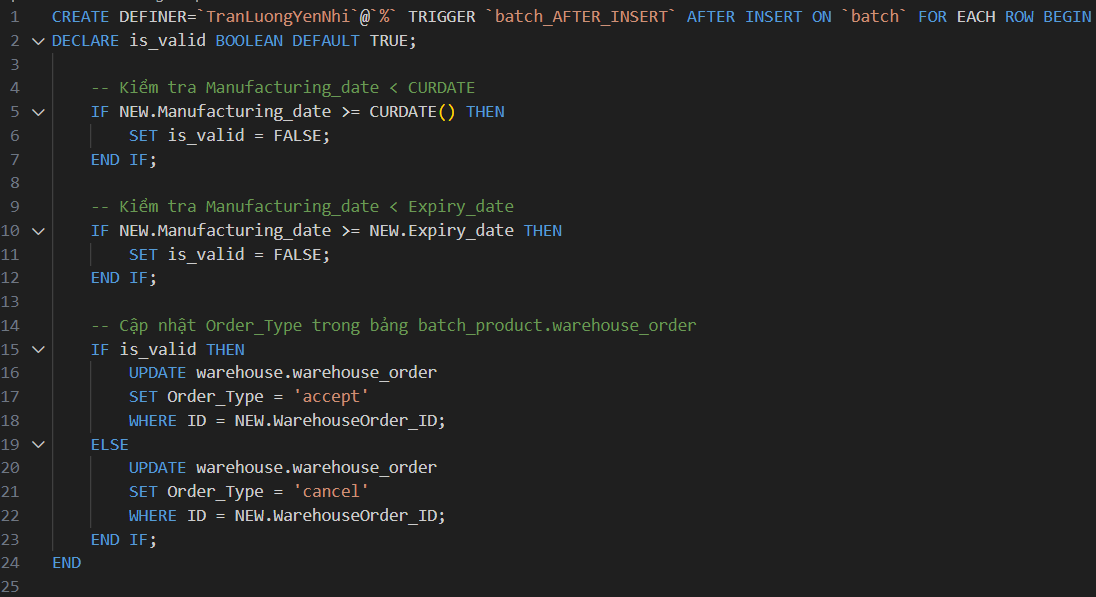
\includegraphics[width=1\linewidth]{trigger.png}
%        \caption{Trigger Batch}
% \end{figure}
\begin{lstlisting}[language=SQL, caption=Tạo trigger cho table Batch] 
CREATE DEFINER=`TranLuongYenNhi`@`%` TRIGGER `batch_AFTER_INSERT` AFTER INSERT ON `batch` FOR EACH ROW BEGIN
DECLARE is_valid BOOLEAN DEFAULT TRUE;

    IF NEW.Manufacturing_date >= CURDATE() THEN
        SET is_valid = FALSE;
    END IF;

    IF NEW.Manufacturing_date >= NEW.Expiry_date THEN
        SET is_valid = FALSE;
    END IF;

    batch_product.warehouse_order
    IF is_valid THEN
        UPDATE warehouse.warehouse_order
        SET Order_Type = 'accept'
        WHERE ID = NEW.WarehouseOrder_ID;
    ELSE
        UPDATE warehouse.warehouse_order
        SET Order_Type = 'cancel'
        WHERE ID = NEW.WarehouseOrder_ID;
    END IF;
END


\end{lstlisting}
Trigger này sẽ kiểm tra xem ngày sản xuất của lô hàng được thêm vào sẽ luôn sớm hơn hoặc bằng ngày hiện tại (thời điểm nhập lô) và hạn sử dụng, sau đó cập nhật trang thái vào đơn kho. Trigger này nhằm để từ chối các lô có thông tin sai lệch (do nhập sai hoặc hàng giả), đảm bảo tính hợp lý của thông tin lô hàng. 